\chapter{Studi Literatur}

Bab ini membahas hasil studi literatur yang diperlukan untuk melakukan
penyusunan Tugas Akhir ini. Bab ini membahas tentang kendaraan otonom, simulator
CARLA, Unreal Engine, Blender, dan penelitian terkait.
%RoadRunner,

\section{Kendaraan Otonom}

Kendaraan otonom atau \textit{Autonomous Vehicle} merupakan kendaraan yang
dirancang untuk memonitor keadaan jalan dan berkemudi sendiri tanpa bantuan
pengemudi. Kendaraan otonom dibuat dengan tujuan mengurangi jumlah kecelakaan,
mengurangi penggunaan energi, mengurangi polusi, mengurangi kemacetan, dan
meningkatkan akses transportasi \parencite{av-bagloee}. Trem otonom sangat mirip
dengan mobil otonom, keduanya beroperasi di lingkungan yang sama dan
berinteraksi dengan objek-objek yang sama pula. Perbedaan keduanya adalah trem
otonom terikat dengan rel trem sehingga trem tidak dapat berbelok keluar dari
rel untuk menghindari objek yang berpotensi menjadi halangan ataupun berhenti
mendadak karena terbatasi secara fisik dan berhenti mendadak dapat mencelakai
penumpang \parencite{at-palmer}.

Trem otonom secara umum memiliki perangkat keras berupa kendaraan fisik,
komputer, dan berbagai sensor. Komputer pada tram digunakan untuk mengoperasikan
trem secara otonom. Komputer juga memiliki kartu grafis untuk melakukan deteksi
objek hasil deteksi dari sensor-sensor di trem. Sensor-sensor tersebut adalah,
kamera, LIDAR, dan radar. Sedangkan pada sisi perangkat lunak, trem otonom pada
umumnya memiliki aplikasi untuk mengolah data sensor \parencite{at-palmer}.

Model pemilihan keputusan oleh kendaraan otonom perlu dilatih sehingga kendaraan
otonom tersebut dapat diandalkan. Oleh karena itu, diperlukan penelitian dan
percobaan lebih lanjut untuk memngembangkan algoritma, kemampuan evaluasi, dan
protokol kendaraan otonom. Penelitan dan eksperimen kendaraan otonom dapat
dilakukan dengan melakukan simulasi detil yang banyak. Simulasi-simulasi
tersebut bergantung kepada model yang ada di dunia nyata \parencite{av-berger}.

Simulasi kendaraan otonom akan memudahkan pelatihan dan proses validasi strategi
kemudi kendaraan otonom. Simulasi mencegah terjadinya kejadian yang berbahaya
dan tidak diinginkan terjadi seperti jika penelitian fisik dilakukan. Penelitian
kendaraan otonom di dunia nyata memiliki banyak rintangan. Penelitian fisik
membutuhkan biaya yang besar untuk membangun kendaraan otonom tersebut,
infrastuktur untuk pengetesan yang memadai, dan biaya lainnya. Selain
dibutuhkannya biaya, dibutuhkan juga sumber daya manusia untuk mengoperasikan
tes. Pengumpulan data juga membutuhkan waktu yang lama karena dibutuhkannya data
yang banyak, data yang valid, dan data yang mencakup kasus-kasus tidak terduga
untuk melatih kendaraan otonom \parencite{carla-dosovitskiy}.

% TODO:
% about tram?
% autonomous vehicles \subsection{Kendaraan Otonom di Indonesia}
% \subsection{Trem Otonom di Indonesia}
% \subsection{Lingkungan Berkendara di Indonesia ?}

% \section{Lingkungan Berkendara di Indonesia}
% street condition, layout, surrounding objects
% \section{Peraturan Lalu Lintas Indonesia}
% traffic rules in Indonesia

\section{Simulator CARLA}

\textit{Car Learning to Act} atau CARLA merupakan sebuah perangkat lunak
\textit{open-source} yang berguna untuk melakukan simulasi kendaraan otonom dan
lingkungan urban. CARLA telah dikembangkan untuk mendukung pelatihan, pembuatan
purwarupa, dan pengujian strategi kemudi otonom, baik dari sisi persepsi maupun
sisi pengontrolan. CARLA menyediakan model dasar untuk lingkungan simulasi,
sejumlah kendaraan, rambu lalu lintas, dan pejalan kaki. Selain itu, CARLA juga
menyediakan keluaran sensor-sensor dan sinyal-sinyal yang dapat digunakan untuk
melatih strategi kemudi seperti koordinat GPS, kecepatan, percepatan, data rinci
mengenai tabrakan yang terjadi pada model kendaraan, dan lain-lain.
Sensor-sensor dan kondisi lingkungan simulasi tersebut dapat diatur sesuai
dengan kebutuhan \parencite{carla-dosovitskiy}.

% \section{\textit{CARLA Simulation Engine}}
CARLA dikembangkan sedemikan rupa sehingga fleksibel untuk disesuaikan dengan
mudah dan juga realistis secara visual dan secara fisika. CARLA diimplementasi
sebagai layar \textit{open-source} di atas Unreal Engine 4 (UE4) sehingga dapat
dikembangkan lebih lanjut oleh komunitas \textit{open-source}.
\textit{Simulation engine} tersebut menyediakan kualitas \textit{render} yang
terkemuka, hukum fisika yang realistis, logika \textit{Non-Playable Character}
(NPC) dasar, dan banyak \textit{plugin} \parencite{carla-dosovitskiy}.

CARLA menyimulasikan sebuah dunia yang dinamis dan juga menyediakan antarmuka
sederhana antara dunia tersebut dan aktor atau agen yang berinteraksi dengan
dunia tersebut. CARLA dirancang sebagai sistem \textit{server-client} sehingga
fungsionalitas tersebut dapat direalisasikan. Server CARLA menjalankan dan
menyimulasikan suasana. Klien bertanggung jawab untuk mengatur interaksi antara
aktor atau agen dengan server via \textit{socket} dengan mengirimkan perintah
untuk aktor dan perintah untuk mengatur peraturan lingkungan simulasi di server.
Klien akan menerima umpan balik hasil rekaman sensor
\parencite{carla-dosovitskiy}.

Lingkungan simulasi pada CARLA terdiri atas model-model 3 dimensi (3D) yang
statik seperti bangungan, tumbuh-tumbuhan, rambu lalu lintas, dan infrastuktur
lainnya. Selain itu, terdapat juga model-model dinamis seperti kendaraan dan
pejalan kaki. Model-model 3D tersebut telah dibuat sehingga dimensi model-model
tersebut mencerminkan dimensi objek aslinya di dunia nyata. Model-model tersebut
dibuat menggunakan model geometrik yang ringan dan dengan tekstur yang sesuai
sehingga terlihat realistis dan detil serta dapat di-\textit{render} dengan
cepat. Aset-aset yang telah disediakan CARLA sangat dapat disesuaikan
\parencite{carla-dosovitskiy}. Aset baru juga dapat ditambahkan
\parencite{carla-documentation-intro}.

% TODO: ? add about how to import or make new assets
% TODO: ? istilah ? add about collision? bounding box blablabla

\section{Unreal Engine}

Unreal Engine merupakan sebuah \textit{game engine} yang dikembangkan oleh Epic
Games. Unreal Engine merupakan sebuah perangkat lunak yang dapat digunakan untuk
membuat permainan, simulasi, dan aplikasi multimedia lainnya. Unreal Engine
memiliki fitur-fitur untuk membuat konten tiga dimensi yang sangat lengkap
\parencite{ue-5}. Jika fitur atau ekosistem Unreal Engine kurang sesuai dengan
kebutuhan pengembang, Unreal Engine menyediakan \textit{source code} yang dapat
dimodifikasi \parencite{ue-4}. CARLA menggunakan Unreal Engine untuk
pengembangan lingkungan simulasi \parencite{carla-documentation-build}.

% TODO: maybe how to add objects?

\section{Blender}

Blender adalah sebuah perangkat lunak \textit{open-source} untuk pembuatan model
3D. Blender dapat digunakan di berbagai sistem operasi dan berjalan lancar pada
Linux, Windows, dan Macintosh. Blender menyediakan berbagai fitur yang mendukung
keseluruhan \textit{pipeline} model 3D. Fitur-fitur tersebut adalah pembuatan
model, \textit{rigging}, pembuatan animasi, pembuatan simulasi,
\textit{rendering}, pembuatan komposit, pelacakan gerakan (\textit{motion
tracking}), pengeditan video, dan pembuatan permainan. Blender menyediakan API
yang dapat digunakan untuk penyesuaian Blender sendiri dan pembuatan alat
pengeditan khusus. API Blender dapat digunakan menggunakan bahasa pemrograman
Python \parencite{blender-about}.

\subsection{Animasi dan \textit{Rigging}}

Animasi adalah membuat sebuah objek
bergerak atau berubah bentuk dari waktu ke waktu. \textit{Rigging} adalah
istilah untuk menambahkan kontrol ke sebuah objek dengan tujuan untuk
menganimasikan objek tersebut. \textit{Rigging} pada umumnya melibatkan komponen
\textit{armature} dan komponen \textit{constraints}. \textit{Armature} berguna
agar objek memiliki sendi yang fleksibel dan sering digunakan untuk animasi
skeletal. \textit{Constraints} adalah batasan dari gerakan objek.
\parencite{blender-animation-and-rigging}.

\subsection{\textit{Armature}}

\textit{Armature} pada Blender merupakan objek yang serupa dengan sistem
kerangka manusia (sistem skeletal) terutama fungsionalitasnya. \textit{Armature}
terdiri atas kumpulan tulang atau \textit{bone} yang memiliki struktur/hierarki
dan berfungsi untuk memberi gerakan ke sebuah objek/model 3D. \textit{Armature}
didesain untuk diberi pose. Gambar \ref{fig:basic-armature} menunjukkan contoh
struktur \textit{armature} sederhana pada Blender. Kumpulan \textit{bone} pada
sebuah \textit{armature} tidak perlu berhubungan satu sama lain sehingga
struktur dari \textit{armature} dapat berupa-rupa, misalnya seperti rantai
tulang atau \textit{chains of bones} yang dapat dilihat pada Gambar
\ref{fig:chains-of-bones} \parencite{blender-armature-introduction,
blender-armature-structure}. Setelah pembuatan \textit{armature} selesai, perlu
dilakukan \textit{skinning} agar pergerakan dari \textit{armature} berdampak
pada objek lain. Proses \textit{skinning} merupakan penghubungan antara objek
\textit{armature} dengan sebuah objek atau objek model/\textit{mesh}
\parencite{blender-skinning-introduction}. Gambar \ref{fig:basic-armature} juga
menunjukkan \textit{armature} yang telah di-\textit{skinning}.

% TODO: find a better way to set counter
\setcounter{section}{1}
\begin{figure}[ht]
    \centering
    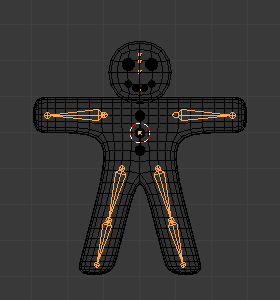
\includegraphics[width=0.4\textwidth]{resources/chapter-2-basic-armature.png}
    \caption{\textit{Skinned armature} sederhana \parencite{blender-armature-structure}}
    \label{fig:basic-armature}
\end{figure}

\begin{figure}[ht]
    \centering
    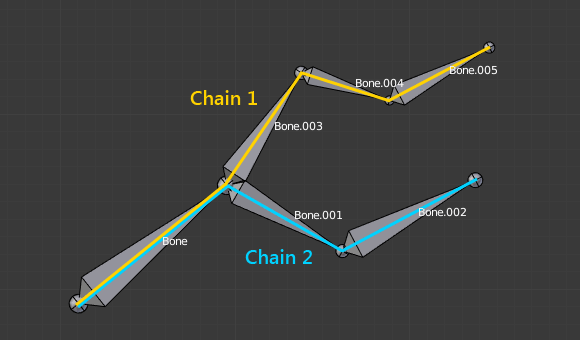
\includegraphics[width=0.6\textwidth]{resources/chapter-2-chain-of-bones.png}
    \caption{\textit{Chains of Bones} \parencite{blender-armature-structure}}
    \label{fig:chains-of-bones}
\end{figure}

\subsection{\textit{Bone}}

\textit{Bone} merupakan komponen dari \textit{armature}
\parencite{blender-bones-introduction}. Struktur sebuah \textit{bone} dapat
dilihat pada Gambar \ref{fig:bone-structure}. Sebuah \textit{bone} terdiri atas
3 subkomponen adalah sebagai berikut:
\parencite{blender-bones-structure,blender-glossary}:

\begin{enumerate}
    \item Sendi awal (\textit{root}/\textit{head})

    Sendi awal memiliki koordinat pada sumbu X, Y, dan Z di ruang lokal
    (\textit{local space}) objek \textit{armature}. Sendi awal merupakan titik
    acuan untuk rotasi \textit{bone} pada sumbu X dan Z pada (\textit{local
    space}). Rotasi ini disebut juga sebagai \textit{roll angle}.

    \item Sendi akhir (\textit{tip}/\textit{tail})

    Sendi akhir memiliki koordinat pada sumbu X, Y, dan Z relatif terhadap sendi
    awal.

    \item Badan (\textit{body})

    Badan oktahedral dari \textit{bone} terbentuk untuk menghubungkan sendi awal
    dan sendi akhir. Bagian sudut oktahedral yang lebih besar berhubungan
    dengan sendi awal. Sebaliknya, bagian sudut oktahedral yang lebih kecil
    berhubungan dengan sendi akhir. Badan \textit{bone} menentukan arah sumbu Y
    lokal dan rotasi \textit{bone} objek ketika diposekan.

\end{enumerate}

\begin{figure}[ht]
    \centering
    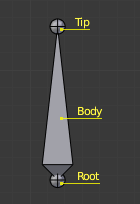
\includegraphics[width=0.3\textwidth]{resources/chapter-2-bone-structure.png}
    \caption{Struktur \textit{bone} \parencite{blender-bones-structure}}
    \label{fig:bone-structure}
\end{figure}

% \section{RoadRunner}
% RoadRunner merupakan sebuah \textit{interactive editor} yang digunakan untuk
% membuat konten desain 3D untuk simulasi dan pengujian sistem kendaraan otonom.
% Pengguna dapat membuat desain jalanan dengan mengedit lingkungan dan menambahkan
% rambu lalu lintas, sinyal lalu lintas, persimpangan, dan batas kendaraan. Selain
% itu, RoadRunner dapat digunakan untuk membuat desain kota \parencite{roadrunner}.

\section{Penelitian Terkait}

Subbab ini membahas beberapa penelitian terkait dengan Tugas Akhir ini.
Penelitian-penelitian berikut menjadi rujukan dalam penelitian dan pengembangan
Tugas Akhir ini.

\subsection{Pengembangan Sistem Otonomi dengan Menggunakan Kecerdasan Artificial untuk Trem}
\label{subsec:rispro-trilaksono}

Penelitian oleh \cite{rispro-trilaksono} merupakan penelitian mengenai inovasi
bidang otomotif yang mengembangkan sistem otonomi untuk Trem menggunakan
kecerdasan buatan. Penelitian tersebut memiliki tiga tahap (dalam tiga tahun)
yaitu, pengembangan \textit{tram driving assistance}, pengembangan trem otonom,
dan pengujian trem otonom di \textit{mixed traffic} serta persiapan
komersialisasi.

Berikut Indikator Kinerja Riset (IKR) atau luaran penelitian tersebut
\parencite{rispro-trilaksono}:

\begin{enumerate}

    \item Pengembangan algoritma persepsi untuk mengenali objek dan
    \textit{tracking} di lingkungan trem pada cuaca normal dan implementasi
    dalam bentuk \textit{software}.

    % Algoritma persepsi yang dikembangkan berupa \textit{panoptic segmentation},
    % \textit{camera object detection}, \textit{LIDAR object detection},
    % \textit{camera-LIDAR fusion object detection}, dan \textit{camera-radar
    % fusion object detection}

    \item Pengembangan algoritma perencanaan jalur untuk \textit{decision
    making} kendali kecepatan trem dan implementasi dalam bentuk
    \textit{software}.

    % Algoritma persepsi yang dikembangkan berupa \textit{railway estimator},
    % \textit{trajectory prediction}, dan \textit{safety assessment}

    \item Pengambilan \textit{dataset} lingkungan trem

    \textit{Dataset} yang diambil bentuk gambar citra kamera biasa, gambar citra
    LIDAR, dan data lainnya kemudian diolah dengan penambahan anotasi
    seperlunya.

    \item Pengembangan \textit{Driving Assistance System} untuk trem berupa:
    \textit{object detection \& collision-avoidance assist}, \textit{speed limit
    assist}, dan \textit{face recognition \& driver attention warning}.

    \item Pengujian, analisis, dan desain ulang algoritma yang dikembangkan pada
    \textit{Software-in-the-Loop Simulation} (SILS) dan
    \textit{Hardware-in-the-Loop Simulation} (HILS).

    Menguji dan menganalisis \textit{platform} simulasi yaitu simulator CARLA
    versi 0.9.12, uji coba beragam sensor, dan uji coba beberapa algoritma yang
    sudah dikembangkan. Melakukan konversi kode program/algoritma yang telah
    dikembangkan ke bahasa pemrograman C++ untuk dimasukkan ke NVIDIA drive AGX
    Pegasus dan membuat \textit{web-service} untuk menghubungkan server simulasi
    (SILS) dengan NVIDIA drive AGX Pegasus (HILS). NVIDIA drive AGX Pegasus
    merupakan \textit{hardware} untuk memroses algoritma \textit{Adaptive Cruise
    Control} (ACC), \textit{Emergency Braking System} (EBS), dan
    \textit{Collision Avoidance} (\textit{decision making}). Dari pengujian dan
    analisis tersebut, dibutuhkan penyempurnaan algoritma persepsi berbasis
    sensor, perbaikan arsitekstur (HILS), dan integrasi objek lokal pada
    skenario simulasi.

    \item Pengembangan dan manufaktur \textit{platform} trem, sistem
    \textit{drive-by-wire} pada trem, dan integrasi sensor.

    \item Publikasi ilmiah.
    \item Draf kekayaan intelektual.
    \item \textit{Self-assessment} Tingkat Kesiapan Teknologi (TKT).
    \item Penyusunan poster ilmiah populer atas pelaksanaan dan hasil riset.

\end{enumerate}

Penelitian tersebut sedang dalam tahap kedua yaitu pengembangan trem otonom.
Masing-masing indikator telah atau sedang dalam perkembangan
\parencite{rispro-trilaksono}. Tugas Akhir \textit{Capstone} ini merupakan
bagian dari penelitian tersebut, khususnya pada indikator mengenai pengembangan
SILS dan HILS.

\subsection{\textit{KIT Bus: A Shuttle Model for CARLA Simulator}}

Penelitian \textit{KIT Bus: A Shuttle Model for CARLA Simulator} ini merupakan
penelitian membuat model \textit{shuttle bus} untuk CARLA yang dilakukan oleh
\cite{related-work-xiang}. Proses pembuatan model tersebut dilakukan dalam tiga
tahap, yaitu sebagai berikut \parencite{related-work-xiang}:

\begin{enumerate}

    \item Membuat model 3D dari bus menggunakan aplikasi 3ds Max.

    Model bus dibuat sesuai dengan referensi dan dimensi asli. Model bus yang
    dibuat secara detil dan berpermukaan mulus sehingga realistis. Model bus
    terdiri atas 6 bagian yaitu, bagian badan, bagian roda-roda, bagian
    interior, bagian detil, bagian kaca, dan bagian plat kendaraan.

    \item Melakukan pengeditan model 3D bus dalam CARLAUE4.

    Model bus yang telah dibuat kemudian diimpor ke dalam CARLAUE4.
    Masing-masing bagian badan bus dan keempat roda bus dipasangkan sebuah
    \textit{collision box} yang berbentuk dan berukuran sama. Agar model bus
    dapat menyimulasikan animasi bus yang sebenarnya, cetak biru animasi harus
    dibuat berbagai macam bagian bus yang bergerak. Dilakukan juga penambahan
    material atau tekstur dan fungsionalitas lainnya yang dibutuhkan seperti,
    lampu dan tekstur-tekstur yang ada pada permukaan bus. Hal tersebut
    dilakukan sehingga model bus dapat menyerupai model bus yang sebenarnya.
    Model bus yang telah selesai diedit dimasukkan ke dalam \textit{vehicle
    factory} agar dapat bisa dimunculkan (\textit{spawn}).

    \item Memverifikasi kontrol manual dan otonom dari model 3D bus yang telah
    dibangun dalam CARLA.

    Model bus yang telah dibuat kemudian diuji untuk memverifikasi apakah model
    bus tersebut dapat dioperasikan secara manual dan otonom. Model bus dites
    untuk berjalan maju, mengerem untuk melambat, mengemudi ke kiri dan ke
    kanan, dan memindahkan gigi kopling.

\end{enumerate}

\subsection{\textit{The Autonomous Siemens Tram}}

Penelitian \textit{The Autonomous Siemens Tram} membahas trem otonom Siemens
yang telah didemonstrasikan di Potsdam, Jerman pada tahun 2018. Sistem trem
otonom tersebut dibangun di atas trem Siemens Combino dan menggunakan
sensor-sensor multi-modal untuk mengidentifikasi lokasi kendaraan serta
mendeteksi dan merespon lampu lalu lintas dan objek lain. Trem otonom memiliki
beberapa komputer yang memiliki \textit{Graphics Processing Unit} (GPU) yang
memadai untuk memroses data dari sensor LIDAR, sensor radar, kamera pendeteksi
objek, dan kamera pendekteksi sinyal. Trem otonom tersebut dapat beroperasi
dengan lancar namun memiliki kendala ketika melakukan lokalisasi trem hanya
dengan Global Navigation Satellite System (GNSS). Penelitian masih dilakukan
untuk mengatasi kendala tersebut, misalnya dengan melakukan lokalisasi dengan
persepsi atau visual \parencite{at-palmer}.
